\newif\iflinenumbers
% Comment in:
\linenumberstrue  % want line numbers
% \linenumbersfalse % want no line numbers

% TODO Clean this up

\documentclass[12pt,oneside,notitlepage,abstracton,a4paper]{article}


% TODO: Find out what these are for
\usepackage{epsfig,scrpage2}
\usepackage{amsmath}
\usepackage{makecell}
\usepackage{graphicx}
\usepackage{booktabs}
\usepackage{arydshln}
\usepackage{setspace} % For singlespace
\usepackage[utf8]{inputenc}
\usepackage[T1]{fontenc}
\usepackage{tablefootnote}

\usepackage{amssymb}  % Equations
\usepackage{xcolor}   % Colours
\usepackage{listings} % Code listings
\usepackage{cancel,xcolor}
\newcommand{\Cancel}[2][black]{{\color{#1}\cancel{\color{black}#2}}}


%%%%%%%%%%%%%%%%%%%%%%%%%%%%%%%%%%%%%%%%%%%%%%%%%%%%%%%%%%%%%%%%%%%%%%%%%%%%%%%%
% Document layout
%%%%%%%%%%%%%%%%%%%%%%%%%%%%%%%%%%%%%%%%%%%%%%%%%%%%%%%%%%%%%%%%%%%%%%%%%%%%%%%%
% TODO Put some order into this part

% For Titlepage
\renewcommand{\headfont}{\normalfont}
  % \cfoot{\pagemark}
  \date{\normalsize \today}
\newcommand{\hwidthline}{
  \noindent\makebox[\linewidth]{\rule{\linewidth}{0.4pt}}
}
%-------------------------------------------------------------------------------
% For TODOS:
\newenvironment{TODOlist}{%
    \begin{list}{\textcolor{DESYorange}{!}\textcolor{DESYcyan}{$\bullet$}\textcolor{DESYorange}{!}}{\setlength{\itemsep}{0.5pt}}
  }{%
    \end{list}%
}

%-------------------------------------------------------------------------------
% To avoid float-only pages change minimum content on page that is necessary
% for page to become float-only
\renewcommand{\floatpagefraction}{.7}

%-------------------------------------------------------------------------------
% For manipulating counters (e.g. figure counter in appendix)
\usepackage{chngcntr}

%-------------------------------------------------------------------------------
% In appendix use the section letter as first numbering letter for everything
\newcommand{\setappendixnumbering}{%
  \renewcommand{\thesection}{\Alph{section}}
  \renewcommand{\theequation}{\thesection.\arabic{equation}}
  \renewcommand{\thefigure}{\thesection.\arabic{figure}}
  \renewcommand{\thetable}{\thesection.\arabic{table}}
  \counterwithin{equation}{section}
  \counterwithin{figure}{section}
  \counterwithin{table}{section}
}

%-------------------------------------------------------------------------------
% Never break footnote onto multiple pages!
\interfootnotelinepenalty=10000

%-------------------------------------------------------------------------------
% Prevent floats to appear below footnotes
\usepackage[bottom]{footmisc}

%-------------------------------------------------------------------------------
% Remove section numbering
% \makeatletter
%   \renewcommand\@seccntformat[1]{}
% \makeatother

%-------------------------------------------------------------------------------
% Add line numbering
%\iflinenumbers
%  \usepackage{lineno}
%  \linenumbers
%\fi

%-------------------------------------------------------------------------------
% For affiliations
\usepackage[affil-it]{authblk}

%-------------------------------------------------------------------------------
% Title page layout (title, authors, affil)
\usepackage{etoolbox} % Tool to modify things (not sure, also need to sort somewhere better...)
\makeatletter % Change Title
\patchcmd{\@maketitle}{\LARGE \@title}{\fontsize{16}{19.2}\selectfont\@title}{}{}
\makeatother
\renewcommand\Authfont{\fontsize{12}{14.4}\selectfont}  % Change author
\renewcommand\Affilfont{\fontsize{9}{10.8}\itshape}     % Change affiliation

%-------------------------------------------------------------------------------
% Smaller side margins
\usepackage{geometry}
\geometry{
 total={170mm,257mm},
 left=20mm,
 top=20mm,
 }

%%%%%%%%%%%%%%%%%%%%%%%%%%%%%%%%%%%%%%%%%%%%%%%%%%%%%%%%%%%%%%%%%%%%%%%%%%%%%%%%
% Directory setup
%%%%%%%%%%%%%%%%%%%%%%%%%%%%%%%%%%%%%%%%%%%%%%%%%%%%%%%%%%%%%%%%%%%%%%%%%%%%%%%%

% Custom paths
\newcommand{\imagepath}{../Plots}
\newcommand{\logopath}{../Logos}
\newcommand{\feynmanpath}{../FeynmanDiagrams}


%%%%%%%%%%%%%%%%%%%%%%%%%%%%%%%%%%%%%%%%%%%%%%%%%%%%%%%%%%%%%%%%%%%%%%%%%%%%%%%%
% Graphics, Figures, Tables
%%%%%%%%%%%%%%%%%%%%%%%%%%%%%%%%%%%%%%%%%%%%%%%%%%%%%%%%%%%%%%%%%%%%%%%%%%%%%%%%

% Custom colors
\usepackage{xcolor}
\definecolor{DESYcyan}{RGB}{0,166,235}
\definecolor{DESYorange}{RGB}{242,142,0}
\definecolor{DESYgray}{RGB}{119,119,119}
\definecolor{bjetpurple}{RGB}{117,112,179}

%-------------------------------------------------------------------------------
% Feynman and other diagrams
\usepackage[compat=1.1.0]{tikz-feynman}
\usepackage{contour}
\usetikzlibrary{arrows,shapes,positioning}
\usetikzlibrary{decorations.markings}
\usetikzlibrary{decorations.pathmorphing}
\usetikzlibrary{decorations.pathreplacing}
\usetikzlibrary{patterns}
\usetikzlibrary{plotmarks}
\usetikzlibrary{shadows}

%-------------------------------------------------------------------------------
% Pretty captions and subcaptions
\usepackage[margin=8mm,font=small,labelfont=bf,format=plain]{caption}
\usepackage[margin=8mm,font=small,labelfont=bf,format=plain]{subcaption}

%-------------------------------------------------------------------------------
% Table top captions and alignment
\captionsetup[table]{position=top}
\captionsetup[subtable]{position=top}

%-------------------------------------------------------------------------------
% Nice features for tables
\usepackage{multirow} % Cells that span multiple rows
\newcommand{\vcell}[3]{\parbox[t]{#1}{\multirow{#2}{*}{\rotatebox[origin=c]{90}{#3}}}}

%-------------------------------------------------------------------------------
% Allows fixing float positions with the [H] option
% \usepackage{float}

%-------------------------------------------------------------------------------
% Shortcut for referencing a subfigure within a figure caption
\newcommand{\subfigref}[1]{({\protect\subref{#1}})}

%-------------------------------------------------------------------------------
% Force floats to appear in its section
% \usepackage[section]{placeins}

%%%%%%%%%%%%%%%%%%%%%%%%%%%%%%%%%%%%%%%%%%%%%%%%%%%%%%%%%%%%%%%%%%%%%%%%%%%%%%%%
% Text manipulation
%%%%%%%%%%%%%%%%%%%%%%%%%%%%%%%%%%%%%%%%%%%%%%%%%%%%%%%%%%%%%%%%%%%%%%%%%%%%%%%%

% Hyperlinks in pdf
\usepackage[
  bookmarks,                   %% PDF-Lesezeichen
  bookmarksopenlevel=1,        %% ...um eine Ebene
  bookmarksnumbered=true,      %% Lesezeichen numerieren
  pdfstartpage={1},            %% mit welcher Seite das PDF öffnen
  pdfstartview={FitH},         %% Zoom auf Seitenbreite
  pdfkeywords={},              %% Stichwörter fürs PDF, kommagetrennt
  pdfsubject={},               %% Themenbeschreibung kurz
  pdfcreator={LaTeX with KOMA-Script and hyperref package},
  hyperfootnotes=true,         %% Links auf Fußnoten
  linkbordercolor={0 1 1},     %% Rahmenfarbe interne Links
  menubordercolor={0 1 1},     %% Rahmenfarbe Literaturlinks
  urlbordercolor={1 0 0}       %% Rahmenfarbe externe Links
]{hyperref}                    %% Hyperlinks und Lesezeichen in PDF



%%%%%%%%%%%%%%%%%%%%%%%%%%%%%%%%%%%%%%%%%%%%%%%%%%%%%%%%%%%%%%%%%%%%%%%%%%%%%%%%
% Additions for math
%%%%%%%%%%%%%%%%%%%%%%%%%%%%%%%%%%%%%%%%%%%%%%%%%%%%%%%%%%%%%%%%%%%%%%%%%%%%%%%%

% Symbols with text above/below
\newcommand{\textover}[2]{\stackrel{\text{#2}}{#1}}
\newcommand{\eqtext}[1]{\textover{=}{#1}} %Equal sign with text over it

%-------------------------------------------------------------------------------
% Dirac notation
\usepackage{slashed}

%-------------------------------------------------------------------------------
% New fancy command for column vector with any number of rows
% (Taken from https://tex.stackexchange.com/questions/2705/typesetting-column-vector)
\newcount\colveccount
\newcommand*\colvec[1]{
        \global\colveccount#1
        \begin{pmatrix}
        \colvecnext
}
\def\colvecnext#1{
        #1
        \global\advance\colveccount-1
        \ifnum\colveccount>0
                \\
                \expandafter\colvecnext
        \else
                \end{pmatrix}
        \fi
}

%%%%%%%%%%%%%%%%%%%%%%%%%%%%%%%%%%%%%%%%%%%%%%%%%%%%%%%%%%%%%%%%%%%%%%%%%%%%%%%%
% Code
%%%%%%%%%%%%%%%%%%%%%%%%%%%%%%%%%%%%%%%%%%%%%%%%%%%%%%%%%%%%%%%%%%%%%%%%%%%%%%%%
% For code snipplet inputs
\usepackage{lmodern}
\usepackage{listings}
\lstset{
  language=[90]Fortran,
  basicstyle=\footnotesize,        % the size of the fonts that are used for the code
  keywordstyle=\color{red},
  commentstyle=\color{green},
  morecomment=[l]{!\ }% Comment only with space after !
  breaklines=true,                 % sets automatic line breaking
  frame=single,	                   % adds a frame around the code
  keepspaces=true,                 % keeps spaces in text, useful for keeping indentation of code (possibly needs columns=flexible)
  % numbers=left,                    % where to put the line-numbers; possible values are (none, left, right)
  % numbersep=5pt,                   % how far the line-numbers are from the code
  % numberstyle=\tiny\color{mygray}, % the style that is used for the line-numbers
  % stepnumber=2,                    % the step between two line-numbers. If it's 1, each line will be numbered
  rulecolor=\color{black},         % if not set, the frame-color may be changed on line-breaks within not-black text (e.g. comments (green here))
  showspaces=false,                % show spaces everywhere adding particular underscores; it overrides 'showstringspaces'
  showstringspaces=false,          % underline spaces within strings only
  showtabs=false,                  % show tabs within strings adding particular underscores
  % tabsize=2,	                   % sets default tabsize to 2 spaces
}


%%%%%%%%%%%%%%%%%%%%%%%%%%%%%%%%%%%%%%%%%%%%%%%%%%%%%%%%%%%%%%%%%%%%%%%%%%%%%%%%
% Bibliography
%%%%%%%%%%%%%%%%%%%%%%%%%%%%%%%%%%%%%%%%%%%%%%%%%%%%%%%%%%%%%%%%%%%%%%%%%%%%%%%%
\usepackage[english]{babel}% Recommended
\usepackage{csquotes}% Recommended
\usepackage[style=numeric-comp,sorting=none]{biblatex}
\addbibresource{library.bib}% Syntax for version >= 1.2

\newcommand{\customprintbibliography}{%
  % \begingroup
  \printbibliography[heading=none]
  % \endgroup
  \newpage
}


%%%%%%%%%%%%%%%%%%%%%%%%%%%%%%%%%%%%%%%%%%%%%%%%%%%%%%%%%%%%%%%%%%%%%%%%%%%%%%%%
% Symbol shortcuts
%%%%%%%%%%%%%%%%%%%%%%%%%%%%%%%%%%%%%%%%%%%%%%%%%%%%%%%%%%%%%%%%%%%%%%%%%%%%%%%%

\usepackage{amssymb}

%-------------------------------------------------------------------------------
% Math/physics symbols
\newcommand{\Lagr}{\mathcal{L}}
\newcommand{\mbar}{\bar{m}}
\newcommand{\oper}{\mathcal{O}}
\newcommand{\DEG}{^{\circ}}

%-------------------------------------------------------------------------------
% Line stuff
\newcommand{\flend}{&&\\} % End of a flalign newenvironment line

%-------------------------------------------------------------------------------
% Particles
\newcommand{\eP}{e^{+}}
\newcommand{\eM}{e^{-}}
\newcommand{\lP}{l^{+}}
\newcommand{\lM}{l^{-}}

\newcommand{\fbar}{\bar{f}}

\newcommand{\eL}{\eM_{L}}
\newcommand{\eR}{\eM_{R}}
\newcommand{\pL}{\eP_{L}}
\newcommand{\pR}{\eP_{R}}

\newcommand{\nue}{\nu_e}
\newcommand{\numu}{\nu_{\mu}}
\newcommand{\nutau}{\nu_{\tau}}
\newcommand{\nul}{\nu_l}

\newcommand{\nubar}{\bar{\nu}}
\newcommand{\nuebar}{\bar{\nue}}
\newcommand{\nulbar}{\bar{\nul}}

\newcommand{\qbar}{\bar{q}}
\newcommand{\qu}{q_{u}}
\newcommand{\qd}{q_{d}}
\newcommand{\qubar}{\bar{q}_{u}}
\newcommand{\qdbar}{\bar{q}_{d}}

\newcommand{\tbar}{\bar{t}}

\newcommand{\vis}{\text{vis}}
\newcommand{\inv}{\text{inv}}

\newcommand{\WP}{W^{+}}
\newcommand{\WM}{W^{-}}

%%%%%%%%%%%%%%%%%%%%%%%%%%%%%%%%%%%%%%%%%%%%%%%%%%%%%%%%%%%%%%%%%%%%%%%%%%%%%%%%
%%%%%%%%%%%%%%%%%%%%%%%%%%%%%%%%%%%%%%%%%%%%%%%%%%%%%%%%%%%%%%%%%%%%%%%%%%%%%%%%










%TODO TO ORDER:
%%%%%%%%%%%%%%%%%%%%%%%%%%%%%%%%%%%%%%%%%%%%%%%%%%%%%%%%%%%%%%%%%%%%%%%%%%%%%%%%

% TODO What is this??
\setcounter{secnumdepth}{3}

\setlength{\parindent}{0em}
\setlength{\parskip}{0ex plus0.5ex minus0ex}
\pagestyle{scrheadings}


%^^^^^^^^^^^^^^^^^^^^^^^^^^^^^^^^^^^^^^^^^^^^^^^^^^^^^^^^^^^^^^^^^^^^^^^^^^^^^^^
% TODO For library execute: chmod u+x combine_bib_entries.sh && ./combine_bib_entries.sh

\begin{document}


%===============================================================================

% Titelpageseite
\begin{titlepage}

  \begin{center}
    \includegraphics[height=3cm]{\logopath/DESY-logo}
  \end{center}

  \vspace{0em}

  \begin{minipage}[t]{\textwidth}

    \begin{minipage}{\linewidth}

      \vspace{0em}

      \begin{center}\bfseries\huge
        Angular efficiency dependance of semileptonic W pair decays at the ILC
      \end{center}

      \vspace{1.0 em}

      \begin{center}\large
        Matthew Koster\\
        University of Cambridge\\
        DESY, Hamburg, Germany\\
        FLC group, Summer Student Programme\\[0.5cm]
        September 4, 2019\\[0.5cm]
        Supervisor: Jakob Beyer
      \end{center}

    \end{minipage}
  \end{minipage}

  \vspace{1cm}

  \begin{abstract}
    It is important to know some angles of stuff for the analysis of the ILD. In this report we discuss how the computation methods required to extrct such angles and stuff. Using kinematic conservation laws to model particles invisible to a particles we are able to extract stuff blah blah blah 

  \end{abstract}

\end{titlepage}

\clearpage

%===============================================================================

\tableofcontents
\clearpage

%===============================================================================

\section{Introduction}
Analysis of the pair production of W bosons in an electron positron collider (see Figure.~\ref{FEY:SemileptonicDecays}) is an important tool for probing the chiral nature of the electroweak interaction for physics Beyond the Standard Model (BSM). A particles chirality is determined by whether the particle transforms in a right- or left-handed representation of the Poincaré group. For massless particles, which travel at the speed of light in all frames, this is equivalent to its helicity which is defined by the projection of the particles spin vector onto its momentum vector. If this projection is positive the helicity is right-handed, and if it is negative the particle is left-handed. Chirality is a bit more subtle for massive particles, because the direction of their momentum is not frame invariant. The charged W bosons only couple to left handed particles and right handed anti-particles, and so the t-channel W pair production mode is only active if the initial state consists of a left-handed electron and right-handed positron (${e}_{L}^{-}{e}_{R}^{+}$). The s-channel, however, is active as long as the electron and position have opposite chirality. This means by adjusting the ratio of ${e}_{L}^{-}$ and ${e}_{R}^{+}$ in the particle beams of a collider, it is possible to switch the t-channel W pair production on and off. This can be used to probe the chiral structure of the electroweak interaction. Furthermore, the triple gauge vertex in the s-channel is a direct consequence of the chiral nature of the electroweak interaction and understanding this W pair production will help us better probe this vertex in a hunt for BSM effects.
\\
\begin{figure}
  \centering
  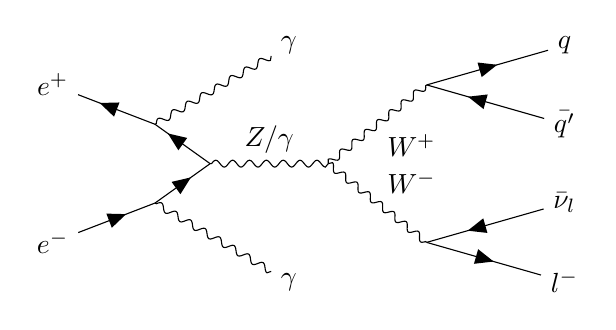
\begin{tikzpicture}
  \begin{feynman}[scale=1] % using the vertex in brackets () allows fixing of vertex
    \vertex (m) at (-1, 0);
    \vertex (n) at (0.5, 0);

    \vertex (r) at (-1.7,-0.5);
    \vertex (s) at (-1.7, 0.5);

    \vertex (a) at (-1.5,-1);s
    \vertex (b) at ( 1.75,-1) ;
    \vertex (c) at (-1.5, 1);
    \vertex (d) at ( 1.75, 1) ;

    \vertex (u) at ( 3.5,-1.5) {$l^-$};
    \vertex (v) at ( 3.5,-0.5) {$\bar{\nu}_l$};

    \vertex (q1) at ( 3.5, 1.5) {$q$};
    \vertex (q2) at ( 3.5, 0.5) {$\bar{q'}$};

    \vertex (i1) at (-3,-1) {$e^-$};
    \vertex (i2) at (-3, 1) {$e^+$};

    \vertex (p1) at (0,-1.5) {$\gamma$};
    \vertex (p2) at (0, 1.5) {$\gamma$};

    \diagram* {
      (i1) -- [fermion] (r) --[fermion] (m) ,
      (i2) -- [anti fermion] (s) -- [anti fermion] (m) ,
      (m) -- [photon, edge label=$Z/\gamma$] (n),
      (b) -- [photon, edge label=$W^-$, swap] (n),
      (d) -- [photon, edge label=$W^+$] (n),
      (b) -- [fermion] (u),
      (b) -- [anti fermion] (v),
      (d) -- [fermion] (q1),
      (d) -- [anti fermion] (q2),
      (r) -- [photon] (p1),
      (s) -- [photon] (p2),
    };
  \end{feynman}
\end{tikzpicture}

  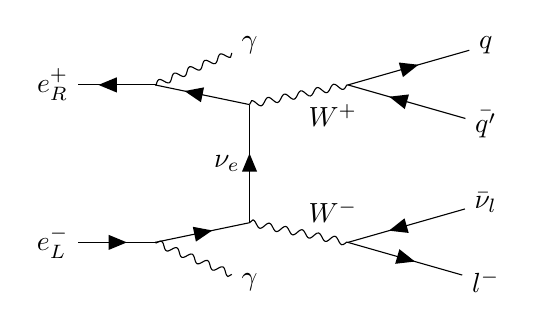
\begin{tikzpicture}
  \begin{feynman}[scale=1] % using the vertex in brackets () allows fixing of vertex
    \vertex (n) at (0, 0.75) ;
    \vertex (m) at (0, -0.75) ;

    \vertex (r) at (-1.2,-1);
    \vertex (s) at (-1.2, 1);

    \vertex (a) at (-1,-1) ;
    \vertex (b) at ( 1.25,-1) ;
    \vertex (c) at (-1, 1);
    \vertex (d) at ( 1.25, 1) ;

    \vertex (u) at ( 3,-1.5) {$l^-$};
    \vertex (v) at ( 3,-0.5) {$\bar{\nu}_l$};

    \vertex (q1) at ( 3, 1.5) {$q$};
    \vertex (q2) at ( 3, 0.5) {$\bar{q'}$};

    \vertex (i1) at (-2.5,-1) {$e_L^-$};
    \vertex (i2) at (-2.5, 1) {$e_R^+$};

    \vertex (p1) at (0,-1.5) {$\gamma$};
    \vertex (p2) at (0, 1.5) {$\gamma$};


    \diagram* {
      (i1) -- [fermion] (r) --[fermion] (m) -- [fermion, edge label=$\nu_e$] (n),
      (i2) -- [anti fermion] (s) -- [anti fermion] (n),
      (b) -- [photon, edge label=$W^-$, swap] (m),
      (d) -- [photon, edge label=$W^+$] (n),
      (b) -- [fermion] (u),
      (b) -- [anti fermion] (v),
      (d) -- [fermion] (q1),
      (d) -- [anti fermion] (q2),
      (r) -- [photon] (p1),
      (s) -- [photon] (p2),

    };
  \end{feynman}
\end{tikzpicture}

  \caption{Lowest order Feynman diagram of semileptonic W pair decay in the $\mu\nubar q\qbar'$ final state at $\eP\eM$ colliders, with two ISR photons emitted. A s-channel (left) and t-channel (right) diagram are shown. Alternately the ${W}^{+}$ could decay leptonically and the ${W}^{-}$ hadronically, which would result in a $\mu^{+}\nu q\qbar'$ final state (not drawn).}
  \label{FEY:SemileptonicDecays}
\end{figure}

The data analysed in this report contains events where an initial state ${e}_{L}^{-}{e}_{R}^{+}$, with a center of mass energy of 500 GeV, produces a pair of W bosons, which in turn decay semileptonically. A semileptonic decay is defined such that one of the W bosons decays leptonically into a lepton and a neutrino, and the other boson decays hadronically into a pair of quarks. In this report, the muon signal of this decay is analysed. From the reconstruction of this interaction, the angular dependence of the detector and reconstruction efficiency is be analysed. This efficiency can then be implemented into the Electroweak Polarisation fit for the International Linear Collider (ILC), which currently assumes a global efficiency value of 60\%, and its effects analysed further.
\\\\\
In Section.~\ref{SEC:MyProcessor} the analysis methods used to extract the 4-momenta information of the final state particles will be discussed, along with a description of the angular distributions that are used. A discussion of how the efficiency of the reconstruction and its angular dependence are evaluated, and how they perform, is conducted in Section.~\ref{SEC:ApplyingCuts}. Finally, the findings of this report are concluded in Section.~\ref{SEC:Conclusion}.


%-------------------------------------------------------------------------------

\section{Example main text section}\label{SEC:Main}

\subsection{Neutrino Reconstruction}
\label{neutrino}
I AM ALWAYS APPLYING CUTS SUCH THAT 1 ISOLEP FOUND AND MC MUONS
\\\\
Pair production of W bosons at $\eP\eM$ colliders is well understood in the Standard Model. These W bosons then proceed to decay and the deacy prodcts leave signals in the detector which are used to analyse the bosons themselves. In my analysis I will be focusing on the semileptonic final state of the W pair decay specifically where the lepton is a muon (Figure.~\ref{FEY:SemileptonicDecays}).
\\\\
\begin{figure}
  \centering
  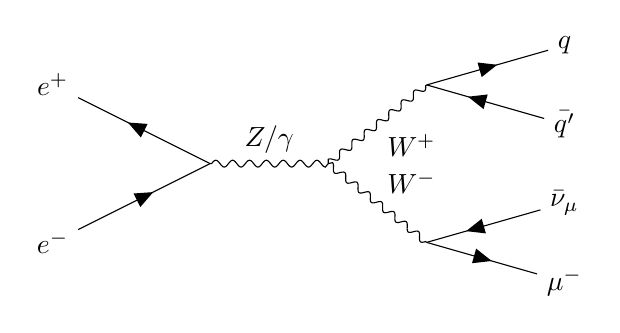
\begin{tikzpicture}
  \begin{feynman}[scale=1] % using the vertex in brackets () allows fixing of vertex
    \vertex (m) at (-1, 0);
    \vertex (n) at (0.5, 0);
    \vertex (a) at (-1.5,-1);s
    \vertex (b) at ( 1.75,-1) ;
    \vertex (c) at (-1.5, 1);
    \vertex (d) at ( 1.75, 1) ;
    \vertex (u) at ( 3.5,-1.5) {$\mu^-$};
    \vertex (v) at ( 3.5,-0.5) {$\bar{\nu}_\mu$};
    \vertex (q1) at ( 3.5, 1.5) {$q$};
    \vertex (q2) at ( 3.5, 0.5) {$\bar{q'}$};
    \vertex (i1) at (-3,-1) {$e^-$};
    \vertex (i2) at (-3, 1) {$e^+$};
    \diagram* {
      (i1) -- [fermion] (m) ,
      (i2) -- [anti fermion] (m) ,
      (m) -- [photon, edge label=$Z/\gamma$] (n),
      (b) -- [photon, edge label=$W^-$, swap] (n),
      (d) -- [photon, edge label=$W^+$] (n),
      (b) -- [fermion] (u),
      (b) -- [anti fermion] (v),
      (d) -- [fermion] (q1),
      (d) -- [anti fermion] (q2),
    };
  \end{feynman}
\end{tikzpicture}

  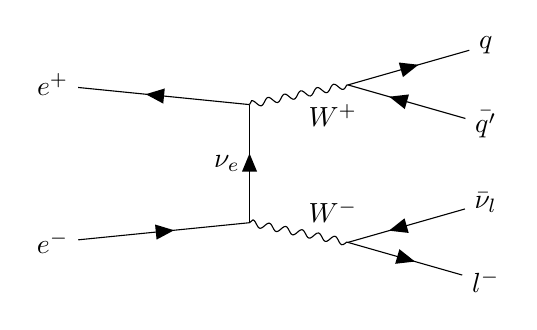
\begin{tikzpicture}
  \begin{feynman}[scale=1] % using the vertex in brackets () allows fixing of vertex
    \vertex (n) at (0, 0.75) ;
    \vertex (m) at (0, -0.75) ;
    \vertex (a) at (-1,-1) ;
    \vertex (b) at ( 1.25,-1) ;
    \vertex (c) at (-1, 1);
    \vertex (d) at ( 1.25, 1) ;
    \vertex (u) at ( 3,-1.5) {$l^-$};
    \vertex (v) at ( 3,-0.5) {$\bar{\nu}_l$};
    \vertex (q1) at ( 3, 1.5) {$q$};
    \vertex (q2) at ( 3, 0.5) {$\bar{q'}$};
    \vertex (i1) at (-2.5,-1) {$e^-$};
    \vertex (i2) at (-2.5, 1) {$e^+$};
    \diagram* {
      (i1) -- [fermion] (m) -- [fermion, edge label=$\nu_e$] (n),
      (i2) -- [anti fermion] (n),
      (b) -- [photon, edge label=$W^-$, swap] (m),
      (d) -- [photon, edge label=$W^+$] (n),
      (b) -- [fermion] (u),
      (b) -- [anti fermion] (v),
      (d) -- [fermion] (q1),
      (d) -- [anti fermion] (q2),
    };
  \end{feynman}
\end{tikzpicture}

  \caption{Lowest order Feynman diagram of semileptonic W pair decay in the $\mu\nubar q\qbar'$ final state at $\eP\eM$ colliders. Alternately the ${W}^{+}$ could decay leptonically, which would result in a $\mu^{+}\nu q\qbar'$ final state (not drawn).}
  \label{FEY:SemileptonicDecays}
\end{figure}

In the MC simulation, there is one hard collision simulated, as well as a bunch of overlay particles, which are importent to model the spectator interstions of the other, non colliding, particles in the bunch. We need to make sure that these extra particles are not included in the reconstruction of the hard intertion. I used 'Fastjet' ***CITE*** processors to remove the overlay from the collection and to find the 2 jets corresponding to the 2 quarks in the final state. I also used the 'MyIsolatedLeptonTagger' ***CITE*** processor to extract the lepton from the recontructed particles. These three extracted particles make up the 'visible' portion of the system. The hadronically decaying W boson can be simply reconstructed by summing the 4-momenta of the 2 extracted quarks it decays into.
\\\\
The leptonically decaying W boson can similarly be reconstructed by summing the 4-momenta of the extracted lepton and the neutrino, however, the neutrino does not leave a signal in the detector. There is also some initial state radiation of photons (ISR) which are aligned enough to the beam pipe that they are lost. This results in an 'invisible' system that is not at all detected by the detector, we must therefore come up with a way to attain the 4-momenta of these invisible particles if we wish to have complete information about the W bosons.
\\\\
The chosen method for reconstruction of the invisible system arises from purely conservation laws\footnote{ a full mathematical derivation is included in the appendix for completeness (\ref{SEC:Appendix})}. We consider the reconstructed visible system as being the hadronically decaying W boson plus the isolated lepton (${p}^{\mu} = ( E,  {p}_{x}, {p}_{y}, {p}_{z})$), and the invisible system as the accompanying neutrino and an ISR photon travelling parallel to the beam. We also assume the total center of mass energy is 500 GeV and that we are in the zero momentum frame (ZMF). Conservation of momentum and energy then gives us the 4-momenta of the ISR photon and the neutrino. In the MC simulation there are actually two ISR photons emitted, this menas that when combining the two photons into one 'photon', this 'photon' may have a non zero invarient mass. The ISR photon could be going in either direction with respect to the beam axis, resulting in two soltuions.
\begin{align}
\label{EQ:full}
{E}_{\gamma}    &= \frac{{\lambda}(500 - E)  \pm {p}_{z}\sqrt{ {\lambda}^{2} - [{(500 - E)}^{2} -{p}_{z}^{2}]{m}_{\gamma}^{2}}}{{(500 - E)}^{2} -   {p}_{z}^{2}}
   \end{align}
 where $ {\lambda} = \frac{1}{2}[{(500 - E)}^2 - {p}^{2} + {m}_{\gamma}^{2} - {m}_{\nu}^{2}] $ has been defined for convenience and no absolute values have been assumed.
\\\\
 My code will then select the solution that gives a better estimate for the invarient mass of the W boson. As described in ***CITE*** this might introduce a bias and so the appropriate cut was made to mitagate this.
\\\\
 It is worth noting at this point that it is numerically possible for the particle reconstruciton to result in a visible 4-momenta with a negative $\lambda$. It can be seen in the ${m}_{\gamma} = {m}_{\nu} =0$ solution that this corresponds to the invisible part of the system having an imaginary invariant mass.
\\
 \begin{align}
 {\lambda}_{{m}_{\gamma}, {m}_{\nu} = 0} \propto {(500 - E)}^2 - {p}^{2} &= {E}_{inv}^2 - {p}_{inv}^{2} = {m}_{inv}^2
      \end{align}
\\
 This is obviously not physical and will affect the solutions attained above. For example as ${p}_{\gamma}= \pm {E}_{\gamma}$,  a negative energy will reverse the direction of the photon. This needs to be handled carefully in the code to avoid inconsistent solutions.
\\\\
 A simplified form of this equaiton with ${m}_{\gamma}= \pm {m}_{\nu} = 0$ is used in the thesis by I.M ***CITE*** that I am basing this analysis on.
 \begin{equation}
   {E}_{\gamma} = \frac{ {(500 - E)}^2 - {p}^{2}}{1000 -2 E  \mp 2{p}_{z}}
\end{equation}
\\\\
In the derivation I show how the full equation above leads to this when simplified, there is however one subtlty when this is done computationally. The $\sqrt{ {\lambda}^{2}}$ will computationally evaluate as $|{\lambda}|$, so if $\lambda$ is negative it will in effect reverse the effect of the $\pm$ in Equation.~\ref{EQ:full} and lead to the opposite solution found using the simplified form. So it is clear that these negative $\lambda$'s may cause some issues.
\\\\
 Using this method I was able to extract the 4-momentum of the leptonically decaying W boson. As a test of the performance of this code I chose to look at the reconstructed invarient mass, to see how accuratly it was reproduced. A peak at around 80 GeV was producted which is close to the currently accepted measurement of 80.3 ***CITE*** which is good, so I explored a few different variables . I found that boosting into the ZMF improved the reconstruction of the mass as is expected (Figure.~\ref{SUBFIG:Boost}). I found that including the true invarent mass of the ISR photon (collected from the simulated MC particle collection performed worse than just setting it to zero (Figure.~\ref{SUBFIG:Mass}).
\\\\
\begin{figure}
  \centering
  \begin{subfigure}[t]{0.45\textwidth}
    \centering
    \includegraphics[width=\textwidth]{\imagepath/Boost.pdf}
    \caption{}
    \label{SUBFIG:Boost}
  \end{subfigure}
  \begin{subfigure}[t]{0.45\textwidth}
    \centering
    \includegraphics[width=\textwidth]{\imagepath/Mass.pdf}
    \caption{}
    \label{SUBFIG:Mass}
  \end{subfigure}
  \caption{
    Plots displaying the effect on the reconstructed invarient mass of the leptonically decaying W with different reconstruction methods.
    The simulated $\eP\eM$ collision is not head on, but with a finite momentum in the x direction, \subfigref{SUBFIG:Boost} shows the effect of boosting into the ZMF before applying the reconstruction method.
    \subfigref{SUBFIG:Mass} shows the effect of inputting a non-zero invarient ISR photon mass into the reconstruction (extracted from the MC collection).
    }
  \label{FIG:MyPlots}
\end{figure}
 I also found that cheating the overlay removal process with the 'TJJetOverlayRemoval' ***CITE*** processor peformed worse than properly using the 'Fastjet' overlay removal (Figure.~\ref{FIG:MyPlots2}). However, when we loot at the reconstruction of the hadronically decaying W boson it performs significantly better.
\\\\
\begin{figure}
    \begin{subfigure}[t]{0.45\textwidth}
      \centering
      \includegraphics[width=\textwidth]{\imagepath/Lep.pdf}
      \caption{}
      \label{SUBFIG:CheatLep}
    \end{subfigure}
    \begin{subfigure}[t]{0.45\textwidth}
      \centering
      \includegraphics[width=\textwidth]{\imagepath/Jet.pdf}
      \caption{}
      \label{SUBFIG:CheatHad}
    \end{subfigure}
    \caption{
      \subfigref{SUBFIG:CheatLep} shows how cheating the overlay removal effects the reconstruction of the leptonically decaying W mass.
      \subfigref{SUBFIG:CheatHad} shows how cheating the overlay removal effects the reconstruction of the hadronically decaying W mass.
      }
    \label{FIG:MyPlots2}
\end{figure}
 Both of these results are slightly concerning as when provided with extra information, that would not be available at a real detector, the reconstruction performs worse than if this extra informaiton is withheld.
\\\\
 In my code I also gave the option for there to be no ISR photon, because there may be some computational issues ***CITE??*** with the formula at low photon energies, and calculated the kinematics as though the only invisible particle was the neutrino. I then observed the effect this had on the boson mass distributions (Figure.~\ref{FIG:STUFF}). It appears that including this options significantly improves the estimations, however I had to check that this isn't just a statistical bais of adding a third possible option to get closer to the true mass. So in Figure.~\ref{FIG:Photon} I plotted the reconstructed photon energy that would have been chosen were there no ${E}_{ISR}=0$ option agains the true MC photon energy, for the events where the full simulation chose the ${E}_{ISR}=0$ option. We see no real correlation forming which is good becuase it means the ${E}_{ISR}=0$ option isnt performing worse, and we see that most of the times when this performed better was at particulatrly low ${E}_{MC}$ values where the formual struggled to get an accurate reconstruction of the photon energy.
 \\\\
 \begin{figure}
   \centering
   \includegraphics[width=\textwidth]{\imagepath/Mass3.pdf}
   \caption{
   Histogram showing how well the 3 different ${E}_{\gamma}$ claculation methods reconstruct the leptonically decaying W mass.
   }
   \label{FIG:STUFF}
 \end{figure}
\begin{figure}
  \centering
  \begin{subfigure}[t]{0.45\textwidth}
    \centering
    \includegraphics[width=\textwidth]{\imagepath/Photon.pdf}
    \caption{}
    \label{SUBFIG:Photon_full}
  \end{subfigure}
  \begin{subfigure}[t]{0.45\textwidth}
    \centering
    \includegraphics[width=\textwidth]{\imagepath/Photon_zoom.pdf}
    \caption{}
    \label{SUBFIG:Photon_zoom}
  \end{subfigure}
  \caption{
    This figure shows the distribution of photon energies from the formula that would have been chosen were there no ${E}_{ISR}=0$ option agains the true MC photon energy, for the events where the full simulation chose the ${E}_{ISR}=0$ option. \subfigref{SUBFIG:Photon_zoom} is the same plot as \subfigref{SUBFIG:Photon_full} with a restricted axis range for clarity.
  }
  \label{FIG:Photon}
\end{figure}

My only current explation for this is that the formula is rather un-sensitive to this change, and so the slight decrease in performance of the ${m}_{W}^{lep}$ estimation is just a statistical fluctuation from the formula.
\\\\
I then apply all of the cuts outlined in I.M. ***CITE*** thesis and see how this effects the selection efficiency. From here on I will be using the method above choosing the best of all 3 possible ${E}_{\gamma}$ solutions with ${m}_{\gamma}= {m}_{\nu} = 0$. Applying the cuts outlined in Table.~\ref{TAB:SelectionEfficiencies}, I arrive at an efficiency flow diagram (Figure.~\ref{FIG:Flow}).
\\\\
  \begin{table}[!]
    \centering
    \caption{
      Selection efficiency of sequantially applied cuts. Where the post ISR correction ${m}_{W}^{lep}$ was calculated using all 3 possible ${E}_{\gamma}$ solutions. (*) Means my and Ivan's cuts differ slightly
    }
    \label{TAB:SelectionEfficiencies}
        \resizebox{0.8\textwidth}{!}{%
        \begin{tabular}{|l|l|l|l|l|} \hline
          Order & Cut description & \multicolumn{3}{c|}{Efficiency [\%]} \\ \cline{3-5}
          & & \multicolumn{2}{c|}{My Results} & Ivan's Results \\  \cline{3-4}
          & & n = 2129 & n = 99419 & n = 107233 \\ \hline \hline
          0 & muon signal & 100.00 & 100.00 & 100.00 \\ \hline
          1 & track multiplicity\tablefootnote{track mulitplicity was taken as the number of reconstructed charged particles.} ${n}_{tracks} \ge 10$ & 97.13 & 97.01 & 99.996 \\ \hline
          2 & center of mass energy $\sqrt{s} > 100$ GeV & 92.29 & 91.69 & 97.96 \\ \hline
          3 & total transverse momentum ${P}_{T} > 5$ GeV & 91.16 & 90.47 & 96.69 \\ \hline
          4 & total energy ${E}_{SUM} < 500$ GeV & 89.66 & 89.28 & 95.36 \\ \hline
          5 & $\ln{({y}_{+})} \in [-12, -3]$ (*) & 88.69 & 88.08 & 95.01 \\ \hline
          6 & 1 lepton found (*) & 80.65 & 80.77 & 78.75 \\ \hline
          7 & pre ISR correction ${m}_{W}^{lep} \in [20, 250]$ GeV &  78.23 & 77.94 & 76.61 \\ \hline
          8 & tau discrimination\tablefootnote{${\tau}_{discr}$ defined by ${\tau}_{discr} = {(\frac{2{E}_{lep}}{\sqrt{s}})}^{2} + {(\frac{{m}_{W}^{lep}}{{m}_{W}^{true}})}^{2}$} &  76.05 & 75.60 &  74.07 \\ \hline
          9 & charged lepton (*) & 76.05 & 75.60 & 73.51 \\ \hline
          10 & isolation variable\tablefootnote{$\Delta{\Omega}_{iso}$ defined as,
          \begin{align}
              ({\phi}_{lep} - {\phi}_{had}) < \pi \to \Delta{\Omega}_{iso} &= \sqrt{{({\theta}_{lep} - {\theta}_{had})}^{2}+{({\phi}_{lep} - {\phi}_{had})}^{2}} \\
              ({\phi}_{lep} - {\phi}_{had}) \ge \pi \to \Delta{\Omega}_{iso} &= \sqrt{{({\theta}_{lep} - {\theta}_{had})}^{2} + {(2\pi - |{\phi}_{lep} - {\phi}_{had} |)}^{2}} \, .
          \end{align}} ${\Delta\Omega}_{iso} > 0.5$ & 76.01 & 75.58 & 73.42 \\ \hline
          11 & post ISR correction ${m}_{W}^{lep} \in [40, 120]$ GeV & 72.90 & 72.77 & 70.13 \\ \hline
          12 & post ISR correction ${m}_{W}^{had} \in [40, 120]$ GeV & 63.21 & 62.92 & 66.93 \\ \hline
          13 & $\cos{{\theta}_{W}} > -0.95$ & 63.02 & 62.65 & 66.78 \\ \hline
        \end{tabular}
        }
    \end{table}

\begin{figure}
    \centering
    \includegraphics[width=\textwidth]{\imagepath/HistFlow.pdf}
    \caption{
    Histogram showing the cut efficiency, with the cut labels defined in Table.~\ref{TAB:SelectionEfficiencies}
    }
    \label{FIG:Flow}
\end{figure}

\subsection{Angle extractions}
\label{angles}
The next part of my project involved extracting a few angles from the hard reaction from the MC Collection. I picked out the semileptonic final state particles from the collection, and reconstructed the leptonic and hadronic jets by basic addition of the 4-momenta. It was then a simple matter of extracting the appropriate angles from the 4 momenta as described in Robert Karls thesis ***CITE*** (Figure.~\ref{FIG:MyPlots2}) from the MC collection.
\\\\
The first angle $\theta_{W^{-}}$ if defined as the angle between the negiativly charged W boson ($W^{-}$) and the beam pipe in the electron direction of travel (the z axis in the MC simuation). I extracted this in the center of mass frame of the $\eP\eM$, which required a boost of $(500\sin{(\frac{0.014}{2})}, 0, 0)$ GeV due to their non zero incidence angle. The rest of the coordinates were simply the polar coordinates of the muon, agian with z aligned to the beam pipe, in the center of mass frame of the leptonically decaying W boson (${\theta}_{l}^{*}$ and ${\phi}_{l}^{*}$) .

\begin{figure}
    \includegraphics[width=\textwidth]{\imagepath/AngleDiag.pdf}
    \caption{
    Angle definition for the 4-fermion final state from ${W}^{-}$ pair production in the semileptonic channel in which the W− decays leptonically. In the top part, the production angles ${\theta}_{{W}^{-}}$ and ${\theta}_{{W}^{+}}$ are defined by the axis of the initial colliding particles and the direction for the respective boson. The azimuthal angles ${\phi}_{{W}^{-}}$ and ${\phi}_{{W}^{+}}$ describe the rotation around the axis of the initial colliding particles.\\
    The bottom picture shows the angular definition of the decay products of the ${W}^{lep}$ boson in its rest frame. It shows the polar angles ${\theta}_{l}^{*}$ and ${\theta}_{\nubar}^{*}$ and the azimuth angles ${\phi}_{l}^{*}$ and ${\phi}_{\nubar}^{*}$ of the corresponding leptons. The ∗ denotes quantities in the rest frame of the ${W}^{lep}$ boson. (Edited from Robert Karl ***CITE***)
      }
    \label{FIG:MyPlots3}
\end{figure}


%-------------------------------------------------------------------------------

\section{Conclusion}
The efficiency of the reconstruction of the semileptonic decay of a W pair produced in an ${e}_{L}^{-}{e}_{R}^{+}$ collision does have an angular dependence that is not currently modelled in the Electroweak Polarisation fit for the ILC. The theta coordinate of the negatively charged W boson, ${\theta}_{{W}^{-}}$, is statistically limited in directions opposite to the initial electron's trajectory and so it is hard to observe the functional form of the efficiency dependance. The efficiency has a clear dependance on the theta coordinate of the lepton in the center of mass frame of the W it decayed from, ${\theta}_{l}^{*}$. There is a drop in efficiency as the leptons direction aligns with the beam pipe. There is no angular dependence observed in the efficiency as the phi coordinate of the lepton in the center of mass frame of the W it decayed from, ${\phi}_{l}^{*}$, is varied.
\\\\
It is also observed that the initial state radiation (ISR) does effect the efficiency of the reconstruction. For events with ISR energies below 1 GeV the reconstruction efficiency is higher by a constant factor, with a similar functional form. As the Electroweak Polarisation fit does not currently model ISR this is an important feature.
\\\\
A significant drop in the efficiency of the reconstruction is due to the beam background removal and due to events where there is no reconstructed isolated lepton, otherwise this reconstruction is seen to perform similarly, and slightly better, than previous studies.
\\\\
In future studies, the potential bias introduced by implementing the three ISR energy solutions in the reconstruction should be looked into and the appropriate cuts made. An alternative approach would be to perform a full kinematic fit to arrive at the best solution for the 4-momenta of the particles in the final state.



%-------------------------------------------------------------------------------

\clearpage

\section{References}
\customprintbibliography

%-------------------------------------------------------------------------------

\clearpage
\section{Acknowledgments}
I would like to thank my supervisor Jakob Beyer for giving me a cool project and always providing instant support whenever I asked for help. Not only this but he provided help to the other summer students in the FLC group without complaint, which went really above and beyond. I'd also like to thank the rest of the FLC group for providing a welcoming environment for us, inviting us on group excursions in and outside of work. Further, Daniel Heuchel and Vladimir Borchanikovn were great office mates and were a pleasure to work alongside.
\\\\
It was great getting to know the other summer students in the FLC group - Sukee Dharani, Andreas Loeshcke Centeno, Peter Mckeown and Lorenzo Cotrozzi. They are all wonderful people and made the long hours writing reports and presentations a lot more bearable, ordering pizza to the office was a terrific idea.
\\\\
I'd like to thank all the summer students who organised group events on the weekends, like our excursions to Cuxhaven and L\"ubeck, and made any food for the community, the cultural food picnic on the last Sunday was fantastic. In particular Jana Wittmann, who organised many events and made many cakes, even delivering one at 5 am!
\\\\
Finally I'd like to thank Olaf Behnke and the organisation team for all their hard work in making this summer programme run smoothly.


%===============================================================================

\clearpage

%-------------------------------------------------------------------------------

\section{Appendix}\label{SEC:Appendix}
\subsection{Log Figures}
\label{App:LogFigures}
\includegraphics[width=0.49\textwidth]{\imagepath/Mass3_log.pdf}
\includegraphics[width=0.49\textwidth]{\imagepath/Mass_log.pdf}

\subsection{Derivation of the ISR energy ${E}_{\gamma}$ with non-trivial ${m}_{\gamma}$ and ${m}_{\nu}$}
\label{App:Derivation}

Our initial assumptions are that the system is in the center of mass frame with an invariant mass of 500 GeV. The system contains a visible 4-momentum ${p}^{\mu} = ( E,  {p}_{x}, {p}_{y}, {p}_{z})$ and an invisible 4-momentum (a neutrino ${p}^{\mu}_{\nu} = ( {E}_{\nu},  {p}_{\nu,x}, {p}_{\nu,y}, {p}_{\nu,z})$ and an ISR photon $ {p}^{\mu}_{\gamma} = ( {E}_{\gamma}, 0, 0,  {p}_{\gamma}) )$. Both the neutrino and the photon have a non trivial invariant mass leading to the following equations.\\\\
Conservation of 3-momentum
\begin{align}
{p}_{x} + {p}_{\nu,x}&=0\\
{p}_{y} + {p}_{\nu,y}&=0\\
{p}_{z} + {p}_{\nu,z} + {p}_{\gamma} &= 0\\
 \end{align}
Conservation of Energy
 \begin{align}
E + {E}_{\nu} + {E}_{\gamma} &= 500
 \end{align}
Energy-Momentum equations
 \begin{align}
{E}_{\nu}^{2} &= {p}_{\nu}^{2} +{m}_{\nu}^{2}\\
{E}_{\gamma}^{2} &= {p}_{\gamma}^{2} +{m}_{\gamma}^{2}\\
 \end{align}
For a unique solution of ${E}_{\gamma}$ we require 2 more constraints on ${m}_{\gamma}$ and ${m}_{\nu}$ which have yet to be imposed, but assuming these constraints are independent of ${E}_{\gamma}$ we can arrive at a solution as follows.\\

From conservation of 3-momentum
 \begin{align}
 {p}_{\nu}^{2} &= {p}_{\nu,x}^{2} + {p}_{\nu,y}^{2} + {p}_{\nu,z}^{2} \\
 					&= {p}_{x}^{2} + {p}_{y}^{2} + {({p}_{\gamma} + {p}_{z})}^{2} \\
 					&= {p}^{2} + {p}_{\gamma}^{2} + 2{p}_{\gamma}{p}_{z} \\
 					&=  {p}^{2} + {E}_{\gamma}^{2} - {m}_{\gamma}^{2} + 2{p}_{\gamma}{p}_{z} \, .
 \end{align}
Conservation of energy then gives us,
 \begin{align}
 {(500 - E)}^2 - {p}^{2} &= {({E}_{\nu} + {E}_{\gamma})}^2  - {p}^{2} \\
 								   &= {E}_{\nu}^{2}  + {E}_{\gamma}^{2} - {p}^{2} + 2{E}_{\gamma}{E}_{\nu}\\
 								   &= {p}_{\nu}^{2}  + {m}_{\nu}^{2} + {E}_{\gamma}^{2} - {p}^{2} + 2{E}_{\gamma}{E}_{\nu}\, .
 \end{align}
Substituting in the expression for ${p}_{\nu}$,
 \begin{align}
{(500 - E)}^2 - {p}^{2} &=  \Cancel[red]{{p}^{2}} + {E}_{\gamma}^{2} - {m}_{\gamma}^{2} + 2{p}_{\gamma}{p}_{z} + {m}_{\nu}^{2} + {E}_{\gamma}^{2} - \Cancel[red]{{p}^{2}} + 2{E}_{\gamma}{E}_{\nu}\\
  {(500 - E)}^2 - {p}^{2} + {m}_{\gamma}^{2} - {m}_{\nu}^{2}
  								&=  2({E}_{\gamma}^{2} + {p}_{\gamma}{p}_{z} + {E}_{\gamma}{E}_{\nu})\\
  								&=  2( \Cancel[red]{{E}_{\gamma}^{2}} + {p}_{\gamma}{p}_{z} + {E}_{\gamma}[500 -  \Cancel[red]{{E}_{\gamma}} - E])\\
  								&=  2( {p}_{\gamma}{p}_{z} + 500{E}_{\gamma} - E{E}_{\gamma} )\, .
 \end{align}
 Where we have one again used conservation of energy.\\\\
 For convenience lets define
\begin{equation}
    {\lambda} = \frac{1}{2}[{(500 - E)}^2 - {p}^{2} + {m}_{\gamma}^{2} - {m}_{\nu}^{2}]
\end{equation}

 and use  ${E}_{\gamma}^{2} = {p}_{\gamma}^{2} +{m}_{\gamma}^{2} $ to arrive at a solvable equation in ${E}_{\gamma} $\, .
  \begin{align}
 {\lambda} &=   {p}_{\gamma}{p}_{z} + 500{E}_{\gamma} - E{E}_{\gamma} \\
  [{\lambda} - (500 - E){E}_{\gamma} ] &=   {p}_{\gamma}{p}_{z} \\
    {[{\lambda} - (500 - E){E}_{\gamma} ]}^{2} &= ({E}_{\gamma}^{2} - {m}_{\gamma}^{2}){p}_{z}^{2} \\
    {\lambda}^{2} - 2{\lambda}(500 - E){E}_{\gamma}  + {(500 - E)}^{2}{{E}_{\gamma}}^{2} &=   {p}_{z}^{2}{E}_{\gamma}^{2} - {p}_{z}^{2}{m}_{\gamma}^{2} \\
        [{(500 - E)}^{2} -   {p}_{z}^{2}]{E}_{\gamma}^{2}  - 2{\lambda}(500 - E){E}_{\gamma} +  ({\lambda}^{2} + {p}_{z}^{2}{m}_{\gamma}^{2})  &= 0
     \end{align}
This can be solved with the quadratic formula to give,
  \begin{align}
 {E}_{\gamma} &= \frac{{\lambda}(500 - E)  \pm \sqrt{ {\lambda}^{2}{(500 - E)}^{2} - [{(500 - E)}^{2} -   {p}_{z}^{2}][{\lambda}^{2} + {p}_{z}^{2}{m}_{\gamma}^{2}] }}{{(500 - E)}^{2} -   {p}_{z}^{2}}\\
 					&= \frac{{\lambda}(500 - E)  \pm {p}_{z}\sqrt{ {\lambda}^{2} - [{(500 - E)}^{2} -   {p}_{z}^{2}]{m}_{\gamma}^{2}}}{{(500 - E)}^{2} -   {p}_{z}^{2}}\, .
     \end{align}
As expected, the solution with ${m}_{\gamma} = {m}_{\nu} =0$  reduces to the previously calculated solution
\begin{align}
 {\lambda} &= \frac{1}{2}[{(500 - E)}^2 - {p}^{2} + \cancelto{0}{{m}_{\gamma}^{2} }- \cancelto{0}{{m}_{\nu}^{2}}]\\
  {E}_{\gamma} &= \frac{{\lambda}(500 - E)  \pm {p}_{z}\sqrt{ {\lambda}^{2} - [{(500 - E)}^{2} -   {p}_{z}^{2}] \cancelto{0}{{m}_{\gamma}^{2}}}}{{(500 - E)}^{2} -   {p}_{z}^{2}}\\
  &= \frac{{\lambda}[(500 - E)  \pm {p}_{z}]}{{(500 - E)}^{2} -   {p}_{z}^{2}} \\
  &= \frac{ \frac{1}{2}[{(500 - E)}^2 - {p}^{2}]}{(500 - E)  \mp {p}_{z}} \\
   &= \frac{ {(500 - E)}^2 - {p}^{2}}{1000 -2 E  \mp 2{p}_{z}}\, .
     \end{align}
  c.f Ivan's result \cite{IvanMarchesini}
  \\
It can also easily be shown for this case that the two solutions correspond to ISR photons travelling parallel or anti-parallel to the z axis. The $\mp$ in the denominator hence corresponds to the sign of the photons z momentum,

\begin{equation}
  {E}_{\gamma} = \frac{ {(500 - E)}^2 - {p}^{2}}{1000 -2 E + 2sgn({p}_{\gamma}) {p}_{z}}
     \end{equation}
\begin{equation}
 {E}_{\gamma} = \frac{{\lambda}(500 - E) + sgn({p}_{\gamma}) {p}_{z}\sqrt{ {\lambda}^{2} - [{(500 - E)}^{2} -   {p}_{z}^{2}]{m}_{\gamma}^{2}}}{{(500 - E)}^{2} -   {p}_{z}^{2}}\, .
     \end{equation}


%===============================================================================

\end{document}

%_______________________________________________________________________________
